\chapter{Measuring a Qubit's State} \label{ch:MeasuringQubitState}

In this chapter, we discuss the basic physics of state measurement in superconducting qubits.
We give a physical and historical picture of state measurement so that the reader will more easily understand the motivation for the work done in this thesis, and the technical details presented in following chapters.

The chapter is divided into three parts.
In the first section we explain why state measurement is generally a hard problem and list the requirements for state measurement in a quantum computer.
In the second section, we discuss the basic measurement mechanisms used in several different types of superconducting qubits.
In the third section, we explain the rationale behind the state measurement mechanism used in the latest superconducting qubits and describe how the work in this thesis was intended to improve upon prior techniques.

\section{Measurement is hard}

Constructing an apparatus to measure the quantum state of a superconducting qubit is inherently difficult.
In order to measure the qubit state, we need to physically couple the qubit to some kind of measurement apparatus, but this introduces unwanted decoherence channels.
A good measurement system must accurately distinguish the quantum states of the qubit on demand, without spoiling the fragile coherence of the state during the coherent control phase of the computation.
Here we list the criteria required of a state measurement system for superconducting qubits.

\begin{enumerate}
\item \textbf{Accuracy:} Existing theoretical protocols for quantum fault tolerance require qubit state measurement with accuracy of at least 90\% if all other parts of the computer, such as the logic gates, operate flawlessly.
However, in a real system with imperfect gates, current protocols require accuracy of $\sim99\%$.
Therefore, we need to be able to distinguish the two computational states $\ket{0}$ and $\ket{1}$ with 99\% accuracy.

The computational states differ by one microwave photon of energy.
Microwave photons, being $10^6$ times less energetic than optical photons, are too low energy to be directly counted with high accuracy.
Energy measurement is therefore not viable, and we have to find other properties of the qubit to use for state discrimination.
Two obvious candidates are the circuit's charge and flux.
If $\ket{0}$ and $\ket{1}$ correspond to different mean values of charge and flux, ie. $\langle \hat{Q} \rangle_0 \neq \langle \hat{Q} \rangle_1$ or $\langle \hat{\Phi} \rangle_0 \neq \langle \hat{\Phi} \rangle_1$, then we can use a charge or flux measurement to distinguish the qubit states.
The charge difference between the qubit states is at most $2e$, and the flux difference is at most $\Phi_0$.\footnote{To give an intuitive idea of these scales we can consider the voltage or current sensitivity needed to measure them. One electron charge on a capacitance of $1\,\textrm{pF}$ gives a voltage of $0.16\mu\textrm{V}$, and larger capacitance, including parasitic capacitance, lower the voltage. One $\Phi_0$ of flux in a $2\,\textrm{pH}$ loop induces $1\textrm{mA}$ of current, and again larger inductance lowers the current.}
Distinguishing these weak signals with the needed accuracy requires exquisitely sensitive and highly specialized detection hardware.
In order to couple to such weak signals the measurement hardware must be integrated onto the same chip as the qubits, meaning that the detector fabrication steps must be compatible with the fabrication of the superconducting qubits themselves.
Despite these difficulties, charge and flux measurement with high accuracy is possible, as we will see below.

The requirement of high accuracy also means that the measurement time must be a small fraction of the qubit lifetime so that the qubit does not change state during the measurement.

\item \textbf{Fast repetition:} In order to be useful in cyclic fault tolerance protocol like the surface code, any reset time in the measurement apparatus must be short compared to the qubit life time. If it is not, then the qubits will lose coherence while the computer waits to be able to use the measurement system.

\item \textbf{Coherence:} The measurement apparatus itself must not spoil the quantum coherence of the qubit states during the coherent part of the computer's operation. The process of measuring a quantum state destroys its coherence by construction, so it is essential that the measurement process can be switched off. If it cannot, then the qubit lifetime can never exceed the measurement time. Furthermore, the measurement system must not inject noise into the qubits or load them with too much damping.\footnote{Injection of noise and damping are actually fundamentally the same thing, as described by the classical and quantum versions of the fluctuation-dissipation theorem. For now, it is useful to think of noise and damping separately for the sake of intuitive reasoning.}

\item \textbf{Non-demolition:} For the purpose of fault tolerance, when measuring a qubit we want to know which state it was in when the measurement was first turned on. Once we have that information, the qubit does not actually have to be in that same state at the end of the measurement. As long as we know which state the qubit was in at the end of the measurement, we can put it into whatever other state we wish with control pulses. A measurement process in which there is a one to one correspondence between the measurement output and the final state of the measured system is said to be ``non-demolition''. A measurement system without this property leaves the qubit in an \emph{unknown} state after measurement, in which case the qubit cannot be reliably reused.

\item \textbf{Multiplexing:} In order for a qubit measurement system to be usable in a quantum computer, it must work not only for single qubits, but for large qubit \emph{systems}. This requirement means that the measurement apparatus should be comparable to or smaller than the the qubits in size, and should not significantly increase the number of control wires needed to operate the computer.
\end{enumerate}

We will keep these criteria in mind as we consider examples of qubit state measurement systems, and comment on how each example does or does not satisfy each criterion.

Note that the criteria presented above and the ensuing discussion are focused on the case of strong projective measurement as appropriate for a surface-code style fault tolerant system.
Other fault tolerance strategies using continuous ``weak'' measurement have been proposed and are the subject of ongoing research.

\section{Examples}

This section discusses a few existing superconducting state measurement systems.
The purpose of the section is to understand the practical difficulties in meeting the criteria given in the previous section, and to get a historical picture of state measurement in superconducting qubits.

\subsection{Charge measurement}

\begin{figure}
\begin{centering}
\includegraphics[width=8cm]{chargeQubit_Nakamura2002.pdf} 
\par\end{centering}
\caption{The charge qubit used in the first time resolved superconducting qubit measurements. (a) Micro-graph of the device in which can be seen the charge reservoir and superconducting island (``box''). The probe electrode on the right is used for charge based state detection. Note the extremely small scale of the device. This was needed so that the self capacitance energy would be much larger than the junction tunnelling energy, which allows charge to be a well-defined (ie. semiclassical) quantity. (b) Schematic of the device showing the geometry of the reservoir, box, and probe electrodes. The image was taken from Ref.\,\cite{Nakamura:qubit2002}.}
\label{Fig:chargeQubit}
\end{figure}

The first time resolved observation of quantum coherence in an electrical circuit was done in 1999 in a charge qubit \cite{Nakamura:qubit1999}.
A charge qubit consists of a superconducting island or ``box'' coupled to charge reservoir (ground) very weakly through a Josephson junction, as shown in Fig.\,\ref{Fig:chargeQubit}.
The $\ket{0}$ and $\ket{1}$ states of the qubit correspond to either zero or one extra Cooper pair having tunnelled from the reservoir to the island.
Because the coupling between the island and ground is so weak, the wave function of the qubit is very narrow in the charge basis, and the charge can be thought of as a well-defined classical variable.
This allows the $\ket{0}$ and $\ket{1}$ states to be distinguished through charge measurement.
A probe electrode is connected weakly to the island through another Josephson junction.
This probe electrode is voltage biased such that when the circuit is in $\ket{1}$ with an extra Cooper pair on the island, two individual electrons can sequentially tunnel out of the island through the probe junction, changing the qubit state from $\ket{1}$ to $\ket{0}$ in the process.
The tunnelling occurs stochastically with a rate set by the parameters of the probe junction and of the qubit.
The slight change in island voltage when the qubit is in $\ket{0}$, combined with the probe bias voltage, blocks electron tunnelling through the probe junction via the Coulomb blockade effect \cite{Nakamura:qubit2002}.
In this way the qubit states were discriminated based on the detection of charge tunneling through the probe junction.

This measurement system has two shortcomings.
First, because the measurement worked through random tunnelling of electrons out of the island, with a corresponding transition of the qubit from $\ket{1}$ to $\ket{0}$, it was by construction a decoherence channel for the qubit.
The probe junction and its associated decoherence channel is always present, so the the excited state of the qubit could never live longer than the rate at which electrons tunnelled out of the island through the probe junction.
This means that the qubit coherence time could not exceed the measurement time.
Second, the measurement required detection of an extremely weak charge signal, just two electrons.
In the original experiment, the authors repeated measurements many times to integrate over many two-electron detections, thus improving the signal to noise ratio enough to distinguish the two qubit states.

In a later experiment, a single electron transistor (SET) was used to detect the charges \cite{Astafiev:singleShot2004}.
The SET is sensitive enough that the visibility of a single-shot measurements was increased to 87\% and 93\% for the $\ket{0}$ and $\ket{1}$ states respectively, bringing the accuracy near the threshold needed for a quantum computer.
The tunnelling process could be turned on and off with voltage biases applied to the readout circuitry, thus satisfying the decoherence criterion.
The measurement circuit needed to be pulsed on for 300\,ns, while the qubit life time was observed up to 5.8\,ns with the measurement off.
Unfortunately, the device had a long reset time of 2\,\textrm{ms}, thus failing the fast repetition criterion.
Furthermore, a single SET was never shown to measure more than a single qubit, and multiplexed readout with a SET is thought to be prohibitively difficult \cite{Yamamoto:private}.

A more fundamental problem is that the charge qubit itself has not been shown to permit the coherence and precise control needed for use in a quantum computer.
Because the wave function is narrow in the charge basis, small noise charges near the qubit lead to random phase noise in the its quantum state, causing loss of coherence.
The charge qubit is so sensitive to charge noise that practical noise levels render it unusable unless it is operated at a specific frequency at which it has a first order insensitivity to charge noise.
Not only is this single frequency operation a major constraint, but the charge noise is so large that even operating at the insensitive point the charge qubit has not yet been shown to permit the degree of control and coherence in a multi-qubit system needed for a quantum computer.
As such it has mostly been abandoned as a candidate for a quantum computer.

\subsection{Flux measurement}

\begin{figure}
\begin{centering}
\includegraphics[width=\textwidth]{fluxQubit.pdf} 
\par\end{centering}
\caption{Potential energy curves and circuit diagram for the flux qubit. a) The flux qubit is a superconducting loop interrupted by three Josephson junctions, one with lower critical current than the other two. An external bias flux $\Phi_{\textrm{ext}}$ controls the shape of the energy potential. b) When the system is biased by an external flux of $\Phi_0 / 2$ the potential is symmetric. In the absence of quantum tunnelling, there would be two degenerate ground states localized within the potential wells, as shown in gray. Tunnelling causes these states to hybridize into symmetric and anti-symmetric states as shown in blue and red respectively. c) When the external flux bias is changed from $\Phi_0 / 2$ (increased or decreased) the degeneracy of the left and right states is removed, and $\ket{0}$ and $\ket{1}$ localize into the left and right wells.}
\label{Fig:fluxQubit}
\end{figure}

\subsubsection{Flux qubit}

In the same year as the first time domain measurements in a charge qubit, quantum behavior was observed in a qubit where the wave function is narrow in the flux basis \cite{Mooij:fluxQubit1999, VanderWal:persistentCurrent2000}.
This qubit, named the ``flux qubit'' uses three junctions\footnote{The use of three junctions instead of just one has to do with design details not covered here. As the junctions are all in series, we can just think of them as a single junction.} in a superconducting loop, as shown in Fig.\,\ref{Fig:fluxQubit}\,a.
When the circuit is biased by an external magnetic flux equal to $\Phi_0 / 2$ the potential takes a symmetric double-well shape.
If the energy barrier separating the two minima were infinitely large, then the system would have two degenerate ground states $\ket{L}$ and $\ket{R}$ as shown by the gray curves in Fig.\,\ref{Fig:fluxQubit}\,b.
With the finite height of the barrier and the nonzero width of the wave functions, the left and right localized states hybridize to form one symmetric and one anti-symmetric state as illustrated by the blue and red curves.
These states are the $\ket{0}$ and $\ket{1}$ states of the qubit.

The qubit states shown in Fig.\,\ref{Fig:fluxQubit}\,b have the same mean flux and charge (the values are zero).
This degeneracy precludes discrimination between the states.
As the degeneracy arises fundamentally from the reflection symmetry of the potential, changing the external bias flux breaks the symmetry, and lifts the degeneracy, as shown in Fig.\,\ref{Fig:fluxQubit}\,c.
A small change in the bias flux causes one well to become lower in energy than the other.
When this happens the hybridization of the two states within the energy wells decreases and the states become more localized.
If this change is made slowly with respect to the frequency of the $\ket{0} \rightarrow \ket{1}$ transition, then the system will remain in whichever energy state it was in initially.
Therefore, if the system starts out in $\ket{0}$, the lower energy state, then after the change in external flux it will be in the left well.
On the other hand, if the system starts out in $\ket{1}$, then after the flux change it will be found in the right well.
The horizontal axis of the plots in Fig.\,\ref{Fig:fluxQubit} is the self flux of the qubit circuit loop, so measurement of magnetic field near the loop yields a measurement of the qubit state.
This strategy was used in Ref.\,\cite{VanderWal:persistentCurrent2000}.

This measurement technique has a major advantage.
The left and right wells are separated by a flux difference of nearly $\Phi_0$, which is a large enough flux to be detected by a superconducting quantum interference device (SQUID) magnetometer with very high signal to noise ratio.
Therefore, the flux qubit state can be measured in a single shot.
Although single shot measurement was not achieved in the original work of Ref. \cite{VanderWal:persistentCurrent2000}, it has become routine in subsequent works using SQUID based measurement.

SQUID readout has several disadvantages.
Operation of a SQUID leads to generation of electrons excited into states above the superconducting gap.
These excited electrons can interact with the qubit mode, so they impose a decoherence channel.
Furthermore, this measurement strategy requires a dedicated SQUID for each qubit, which complicates scaling to larger systems.

\subsubsection{Phase qubit}

\begin{figure}
\begin{centering}
\includegraphics[width=\textwidth]{phaseQubit.pdf} 
\par\end{centering}
\caption{The phase qubit. a) The phase qubit is operated such that the wave function sits in an asymmetric shallow well of the potential energy. Tunneling out of this well is used as a mechanism for measurement. b) The ground (blue) and excited (red) states in the shallow well are meta-stable. By momentarily lowering the height of the potential barrier, the excited state tunnels out of the well, while the ground state remains in the well. c) Once the excited state has tunneled, external bias is used to bring the potential into a symmetric shape where the states are separated by a large flux and can be measured with a SQUID.}
\label{Fig:phaseQubit}
\end{figure}

Another double-well qubit, the ``phase qubit'' was introduced in 2002 \cite{Martinis:rabi2002}.
The wave functions of the phase qubit are so narrow in the flux basis that they would not normally feel enough of the anharmonic shape of the potential wells to behave with the non-linear character needed for a qubit.
To recover the non-linearity, a bias (current in the original work, but flux in later versions) introduces asymmetry in the potential, making one of the wells very shallow, as shown in Fig\,\ref{Fig:phaseQubit}\,b.
In this arrangement, the wave function feels the asymmetric potential shape enough to form unequally spaced levels.
The two logical states of the qubit are the ground and first excited states of this shallow well.

To measure the state, we selectively tunnel the the excited state into the right potential well, as shown in Fig.\,\ref{Fig:phaseQubit}.
A short bias pulse is used to momentarily lower the height of the barrier seen in Fig.\,\ref{Fig:phaseQubit}\,b.
This allows the excited state to tunnel out of the shallow left hand well and fall into the deep right hand well.
The ground state remains in the left hand well.
The bias is then changed to bring the potential into the symmetric shape shown in Fig\,\ref{Fig:phaseQubit}\,c where the two states can be distinguished by their now different fluxes using a SQUID.

The benefit of this measurement strategy is that the states can be distinguished with $>90\%$ accuracy using a very fast measurement pulse.
However, there are several drawbacks.
First, the decay of the tunneled excited state to the bottom of the right hand well is a dissipative process.
Emission of energy during this process has been observed to drive neighboring qubits into excited states, causing measurement cross-talk errors.
Second, the process of tunneling into the right hand well renders the phase qubit no longer a qubit: it has undergone fundamentally dissipative evolution, destroying its phase coherence, and it no longer resides in the shallow nonlinear well.
This means that a phase qubit measured in this way cannot be used to store and process quantum data in a protocol requiring more than one measurement step, such as the surface code.
Note, however, that the phase qubit could still be used as a measurement device by mapping the state of a data qubit onto the phase qubit and then measuring the phase qubit.
This idea is discussed further below.
In any case, once the phase qubit tunnels, it must be reset into the shallow well if it is to be used again.
This is complicated by the fact that we may not know whether or not the phase qubit tunneled.
Practical reset times for the phase qubit are in the tens to hundreds of microseconds, which is much too long compared to the coherence times of currently available devices.

\subsection{Inductance measurement}

\begin{figure}
\begin{centering}
\includegraphics[width=10cm]{quantronium.pdf} 
\par\end{centering}
\caption{The quantronium qubit. The leftmost branch is essentially a charge qubit with two junctions connecting the island to the reservoir. The extra capacitance in the next branch reduces the quantronium's sensitivity to change noise. The rightmost three branches, shown in dotted line, are used for measurement. With the current source off, the circuit mode is symmetric from top to bottom and does not couple into the amplifier or large junction. Turning on the current bias breaks this symmetry, and when the large junction switches to the voltage state that voltage is measured by the amplifier.}
\label{Fig:quantronium}
\end{figure}

Also in 2002 a superconducting qubit called the ``quantronium'' was introduced \cite{Vion:quantronium2002}.
This device has characteristics in between those of the charge and flux qubits.
A circuit diagram of the quantronium is shown in Fig.\,\ref{Fig:quantronium}.
Focusing first on the part of the circuit drawn with solid line, the device is essentially a charge qubit: a superconducting island coupled to a charge reservoir through a junction, but here the single junction of the charge qubit is replaced by a nominally symmetric pair of junctions.
This branch is shunted by a parallel capacitance.
The additional capacitance causes the qubit wave function to broaden in the charge basis while simultaneously narrowing in the flux basis, which reduces sensitivity to charge noise.\footnote{Reduced charge noise incurs increased flux noise, but with the parameters used at the time this change lead to an over-all improvement in the device performance.}
Note that due to the symmetry of the circuit, the qubit mode has equal voltage on the top and bottom (points A and B in Fig.\,\ref{Fig:quantronium}).

The quantronium uses an integrated measurement circuit, as illustrated by dotted part of Fig.\,\ref{Fig:quantronium}.
The measurement circuit consists of a large Josephson junction, a current source, and a voltage amplifier connected in parallel with the qubit.
In normal operation the current bias current is set to zero, and in that case, because of the symmetry of the circuit, the qubit oscillation mode couples neither to the large junction nor to the amplifier.
This prevents the readout circuit from loading the qubit with a decoherence channel.

To measure the state of the quantronium, the bias current is pulsed on.
The current pulse divides between the branch with the small junctions and the branch with the large junction.
The pulse height is nearly the critical current of the large junction.
Depending on the state of the qubit, the inductance of the small junctions will be slightly different, and additional current may flow into the large junction, causing the total current to exceed the large junction's critical current.
This causes the large junction to switch out of the superconducting state and produce a voltage pulse which is detected by the amplifier.
The important feature of this system is that the readout circuitry does not couple to the qubit mode during normal operation.
Only when the current source is turned on does the qubit mode couple to the readout circuit.
This prevents the readout system from introducing unwanted decoherence into the qubit while the measurement system is off.

Still, this system has disadvantages.
Exceeding the large junction's critical current to produce a voltage signal generates electron excitations above the superconducting gap, just like the SQUID used to measure flux qubits.
Additionally, this system requires a bias current line and voltage amplifier for every qubit, which would bring a large and difficult to engineer overhead into design of a quantum computer.
However, as is the case with the charge qubit, the most important problem is that control of the quantum state of quantronium qubits has not been demonstrated to be accurate enough to effect the single and multiple qubit logic gates needed for a quantum computer.

Note that this system does not directly measure charge or flux. The switching of the large junction depends on the qubit state through the intrinsic inductance of the small junctions, rather than on a electric or magnetic field produced by the circuit.

\section{The transmon qubit - RF measurement}

\begin{figure}
\begin{centering}
\includegraphics[width=10cm]{transmon_2.pdf} 
\par\end{centering}
\caption{The transmon circuit and energy potential. a) The transmon is similar to a parallel LC oscillator, but with a nonlinear inductor. The potential energy has the shape of a cosine, and the large $C$, analogous to a large mass, prevents the wave functions from tunneling between wells. b) The single junction is replaced by a loop with a pair of junctions. External flux is used to modulate the effective critical current of the loop, which changes the height of the potential energy. This in turn causes the resonance frequency to shift.}
\label{Fig:transmon}
\end{figure}

As of this writing, the only superconducting qubit which has been demonstrated to support high accuracy control in single and two qubit logic gates is the transmon \cite{Koch:transmon2007, Barends:gates2014}.
The basic transmon circuit is shown in Fig.\,\ref{Fig:transmon}\,a.
It is essentially an LC oscillator, but with a Josephson junction in place of a normal inductor to make it non-linear.
This is precisely the simple circuit we considered in Chapter \ref{ch:Introduction} with the Hamiltonian \begin{equation}
H = \frac{Q^2}{2C} - E_J \cos \left( 2\pi \Phi / \Phi_0 \right), \quad [\Phi, Q]=i\hbar. \end{equation}
The first term is completely analogous to the kinetic energy of a mechanical system $T = p^2 / 2m$ if we think of $Q$ as the momentum and $C$ as the mass.
Similarly, we can think of $\Phi$ as the position of the particle in a cosine shaped potential energy with height $E_J$.
Noting that in the mechanical case $[x,p]=i\hbar$ completes the analogy.
The transmon is designed with a large $C$ to make it insensitive to charge noise.
This, being equivalent to a large mass, prevents the wave function from tunneling between the minima of the cosine potential.
As a result, we can consider only a single minimum, as indicated by the solid line part of the potential in Fig.\,\ref{Fig:transmon}\,a.

In practice the single junction is replaced by a pair of junctions in a loop, as illustrated in Fig.\,\ref{Fig:transmon}\,b.
This allows the resonance frequency of the transmon to be modulated dynamically.
The loop acts like a single junction, but with a critical current $I_c$ which depends on external flux threading the loop.
Because the inductance of a junction is related to the critical current by $L_J = L_{J_0}/\sqrt{1 - \left( I/I_c \right)^2}$, we can control the inductance, and therefore the resonance frequency $\omega_{0}$ of the circuit, via the external flux.
Another way to think about this is that the external flux changes the effective $E_J$ of the two-junction loop, thus changing the height of the cosine potential, as illustrated in Fig.\,\ref{Fig:transmon}\,b.
This change in the shape of the potential causes the energy difference between the states to change, thus changing their resonance frequency.

The transmon is particularly difficult to measure.
Like the flux qubit the wave functions are broad in the charge basis, so the states cannot be distinguished via charge detection.
On the other hand, because of the symmetric shape of the potential the states all have the same mean flux.
Therefore, charge-based and flux-based measurements are both impossible.

\subsection{Qubit as a photo-detector}

One measurement strategy is to transfer the transmon state into a different kind of qubit where charge or flux measurement is available.
This idea, which is essentially using a qubit as a microwave photon detector, is illustrated in Fig.\,\ref{Fig:swapMeasurement}.
The measurement process is turned on by dynamically tuning the transmon into resonance with the detector, in this case a phase qubit.
If there is a quantum of energy in the transmon, then when the transmon comes on resonance with the phase qubit, the photon begins to oscillate between the two qubits.
Once the photon is completely swapped into the phase qubit, the transmon is taken off resonance to stop the interaction.
The phase qubit is then measured in the normal way.
If the phase qubit is measured to be in the excited state, then there must have been a photon collected from the transmon and so the initial state of the transmon is inferred by the measured state of the phase qubit.

This strategy does work, and in fact was used in the initial transmon experiments at UCSB.
However, it inherits all of the problems already mentioned with phase qubit measurement, most importantly the long dead time needed to reset the phase qubit.

\begin{figure}
\begin{centering}
\includegraphics[width=10cm]{swapMeasurement.pdf} 
\par\end{centering}
\caption{Qubit measurement by swapping the excitation into an auxiliary circuit. (a) The qubit starts in a superposition of the ground (blue) and excited (red) states. (b) The qubit is brought on resonance with the detector. If it was in the excited state, one quantum of energy is swapped into the detector, otherwise nothing happens. In either case, the qubit is left in the ground state. (c) The qubit is brought off resonance with the detector to turn the interaction off. The detector is now in one of two measurably different states corresponding to the two possible qubit states.}
\label{Fig:swapMeasurement}
\end{figure}

\subsection{Energy measurement with travelling waves}

We consider briefly the notion of directly measuring the qubit energy, as it will shed light on the subsequent discussion.
Suppose we allow the qubit energy to leak out from the qubit into an amplifier as a travelling wave, using a circuit as shown in Fig.\,\ref{Fig:waveMeasurement}\,a.
The qubit state would then be determined by measuring the amplitude of the wave after the amplifier by conventional means.
Crucially, many qubits could be attached in parallel to the same transmission line and amplifier with the various output signals discriminated via frequency multiplexing.
The problem with this solution is that the signal to noise ratio is fundamentally limited to near unity.
The theoretical limit on the input referred noise power of a phase preserving linear amplifier is $P_N = (1/2)\hbar \omega B$ where $B$ is the amplifier bandwidth \cite{Caves:amplifiers1982}.\footnote{We consider linear amplifiers because we want frequency multiplexing.}
For a measurement of duration $T$, the collected noise energy would be $E_N = P_N T = (1/2)\hbar \omega B T$.
To measure a pulse of length $T$ the amplifier bandwidth must satisfy $B \gtrapprox 1/T$, so $E_N \gtrapprox (1/2) \hbar \omega$.
This is already half as large as the maximum energy that could be collected from the qubit in a system with perfect efficiency.
Therefore, the signal to noise ratio fundamentally cannot exceed 2, which is too low.
The intrinsic suitability of this circuit for scaling to larger numbers of qubits suggests we find a way to fix the signal to noise ratio problem.

\begin{figure}
\begin{centering}
\includegraphics[width=10cm]{waveMeasurement_2.pdf} 
\par\end{centering}
\caption{Measurement based on traveling waves. a) The qubit state is determined by the presence or absence of an outgoing wave. As the maximum measured energy is just the single photon in the qubit, the signal to noise ratio is too low. b,c) An externally supplied voltage is used to raise the signal to noise ratio. The wave acquires a qubit state dependent phase shift as it scatters from the shunt line containing the qubit. The blue and red curves indicate the phase response for the qubit in $\ket{0}$ and $\ket{1}$, respectively. The gray curve indicates the difference in these phases. The center frequencies of the qubit in the ground and excited states are indicated by the blue and red arrows, and the frequency yielding the maximum phase signal is indicated by the black arrow. d,e) A filter placed between the qubit and external resistance could raise the limit on qubit lifetime, but this leads to a smaller detectable phase shift.}
\label{Fig:waveMeasurement}
\end{figure}

\subsection{Dispersive measurement}

As we can measure neither the charge, flux, nor energy, we need to find another parameter of the qubit that differs between the two states.
Because the qubit is non-linear its resonance characteristics depend on its energy state.
This suggests that a spectroscopic measurement might be possible.
Think of the qubit as a simple harmonic oscillator, but whose resonance frequency depends on whether it is in $\ket{0}$ or $\ket{1}$.
As a probe signal applied to the circuit is swept in frequency, the phase shift acquired by that signal undergoes a sharp change across the resonance.
As this resonance frequency depends on the qubit state, we can use the position of the phase shift to measure the qubit.
A circuit diagram suitable for this measurement is shown in Fig.\,\ref{Fig:waveMeasurement}\,b.
The probe signal is injected into the left side of the transmission line.
As it travels past the qubit and drives the qubit resonance, it picks up a phase shift which depends on the qubit state.
The phase responses for the two states are plotted in Fig.\,\ref{Fig:waveMeasurement}\,c.
By probing at a frequency between the two possible qubit resonances, the phase shift difference is maximized and the qubit state could be determined.

This strategy solves the signal to noise ratio problem because the energy of the injected wave can be arbitrarily large.
However, we have a coherence problem because the resistance in the external circuitry loads the qubit.
In fact, the qubit lifetime imposed by this external circuitry is equal to the time it takes for the qubit to respond to the probe pulse and react with a phase shift.
This means that the qubit life time during the measurement cannot significantly exceed the measurement time.

We could try to isolate the qubit from the damping of the external circuit with a filter, as illustrated in Fig.\,\ref{Fig:waveMeasurement}\,d.
The filter decouples the qubit circuit from the external circuit over a frequency range including the qubit resonance, so the qubit is not damped.
However, the filter also decouples our probe signal from the qubit in that frequency band, so we would have to probe outside the band blocked by the filter.
Far from the qubit resonance, the phase acquired by the probe signal is insensitive to the qubit state, as shown in Fig.\,\ref{Fig:waveMeasurement}\,e, so the states are not well discriminated.

To isolate the qubit from damping while still allowing the probe signal to acquire a state dependent phase shift, we replace the filter in Fig\,\ref{Fig:waveMeasurement}\,d with an auxiliary harmonic resonator, as shown in Fig.\,\ref{Fig:resonatorMeasurement}\,a.
The resonator frequency $\omega_r$ is detuned from the qubit by a frequency $\Delta$.
Therefore, \emph{at the qubit frequency} the resonator is a short to ground and prevents the qubit from feeling the dissipation of the external circuitry.
This blocks radiation from the qubit, and solves the coherence problem.
As the qubit has different impedance in its two states, the loading it imparts on the resonator is state dependent, so the resonator frequency depends on the qubit state.
We characterize the resonator frequency shift by a parameter $\chi$, defined by $2 \chi = \omega_{r,\ket{0}} - \omega_{r,\ket{1}}$, as shown in Fig.\,\ref{Fig:resonatorMeasurement}\,b.
We infer the qubit state by probing the system in between the two resonator frequencies and measuring the phase.

\begin{figure}
\begin{centering}
\includegraphics[width=\textwidth]{resonatorMeasurement.pdf} 
\par\end{centering}
\caption{Schematic for measurement with an auxiliary resonator. a) The qubit is protected from resistance in the external circuitry by a detuned resonator which acts as a short at the qubit frequency. b) The qubit states cause the resonator frequency to shift, leading to large measureable phase shift at the resonator frequency.}
\label{Fig:resonatorMeasurement}
\end{figure}

The physics of the qubit state-dependent resonator frequency shift was first demonstrated in 2004 and 2005 at Yale with charge qubits \cite{Schuster:acStarkDephasing2005, Wallraff:2004, Wallraff:unitVisibility2005}, and the shift was first used to measure qubit states in those experiments.
This strategy has been named ``dispersive measurement'' or ``dispersive readout'' because it depends on the qubit state dependent dispersion of the probe signal.
Using bifurcation amplifiers, dispersive measurement was shown in 2009 to yield measurement with accuracy up to 94\% \cite{Mallet:singleShot2009}, and later experiments with transmon qubits using linear Josephson parametric amplifiers achieved accuracy up to about 94\% \cite{Johnson:heralding2012}.

The dispersive measurement strategy does have an important limitation. We said above that the resonator blocks the qubit from feeling the dissipation of the external circuitry, but this is true only up to a point.
Even far off resonance, the resonator is not a perfect short, so the qubit is still damped to some degree.
This effect is quantified by a relation between four parameters.
First, we have the limit on qubit lifetime $T_1$ imposed by the measurement circuit.
Second, we have the resonator-transmission line coupling strength characterized by the inverse ring-up time $\kappa_r$.
This is set by $C_{\kappa}$, as shown in Fig.\,\ref{Fig:resonatorMeasurement}.
Next is the the resonator-qubit coupling strength $g$, which is set by $C_g$, as shown in Fig.\,\ref{Fig:resonatorMeasurement}.
Finally, we have the qubit-resonator detuning $\Delta$.
These parameters are related by \cite{Blais:cQED2004} \begin{equation}
\kappa_r T_1 \lesssim \left( \frac{\Delta}{g} \right) ^2 . \label{eq:simplePurcell} \end{equation}
This formula expresses a tension between fast response time of the resonator $\kappa_r$ and long coherence time of the qubit $T_1$.
For a given $\Delta$ and $g$, speeding up the measurement with faster $\kappa_r$ leads to lower $T_1$ of the qubit.
As shown in Chapter \ref{ch:DispersiveMeasurement}, to get a large measurable phase shift, there is an additional constraint \begin{equation}
\kappa_r \approx \chi = \frac{g^2}{\Delta} \label{eq:simpleChiMatch} \end{equation}
which comes from the fact that, because the resonator is attached in parallel with the transmission line, the phase response measured in the circuit shown in Fig.\,\ref{Fig:resonatorMeasurement}\,a is not actually the pure arc tangent shown in Fig.\,\ref{Fig:resonatorMeasurement}\,b. Combining equations (\ref{eq:simplePurcell}) and (\ref{eq:simpleChiMatch}) yields \begin{equation}
\kappa_r^2 T_1 \lesssim \Delta . \end{equation}
Suppose we have a qubit with an intrinsic energy decay time of $T_1$.
For 99\% accurate measurement we need the entire measurement procedure to be shorter than $T_1/100$.
Taking the entire measurement sequence to require a time of $10\kappa_r^{-1}$, this means we need $\kappa_r^{-1} \geq T_1 / 1000$.
With currently available transmons at $T_1 \approx 20-40\,\mu\textrm{s}$, this gives $\kappa_r^{-1} \sim 30\,\textrm{ns}$ and therefore requires $\Delta > \kappa_r^2 T_1 = 30\,\textrm{GHz}$.
This large of a qubit-resonator detuning is completely impractical.
With the qubit at $\sim 6\,\text{GHz}$, such a large $\Delta$ would put the resonator at such a high frequency that practical microwave engineering becomes much more difficult.
For example, parasitic resonances on the micro-fabricated qubit chips become a serious problem when the signal wavelength becomes smaller than the size of the chip.
A frequency of $30\,\textrm{GHz}$ corresponds to a wavelength of $1\,\textrm{cm}$ in vacuum (substantially less in a dielectric substrate) which is on the order of practical chip sizes.
Another strategy is needed.

\subsection{Filters}

\begin{figure}
\begin{centering}
\includegraphics[width=0.8\textwidth]{yaleFilter.pdf} 
\par\end{centering}
\caption{A filter used to increase the $\kappa_r T_1$ product. a) The filter is placed on the output of the resonator to prevent radiation at the qubit frequency from leaving the system. b) The filter was implemented as a symmetric pair of $\lambda/4$ stubs to ground. c) Micrograph of the Yale device. The filter is seen on the right side as two meandering co-planar wave guide resonators. d) Transmission through the system. Note the notch just above $6\,\textrm{GHz}$, which protects the qubit. The large increase in transmission at 8\,GHz is the resonance frequency of the resonator.}
\label{Fig:yaleFilter}
\end{figure}

In 2010, researchers at Yale introduced the idea of on-chip filters to further protect the qubit from damping induced by environment \cite{Reed:filter2010}.
The circuit is shown in Fig.\,\ref{Fig:yaleFilter}\,a.
In this system the resonator is constructed from a $\lambda/2$ piece of co-planar wave guide inserted in series with the drive line.
The qubit is connected in parallel with the resonator, and the filter is placed on the output of the resonator.
This filter forms a notch at which energy cannot leave the resonator.
By placing this notch at the qubit frequency, the qubit is protected from emitting energy.
In Ref.\,\cite{Reed:filter2010}, it was shown that for a given $\Delta$, $\kappa_r$, and $g$, the filter increased the qubit $T_1$ above the limit from Eq.\,(\ref{eq:simplePurcell}).
However, that work did not discuss the all important speed and accuracy of the measurement.

Introduction of on-chip filters was a big step forward for measurement of superconducting qubits, because it opened the door for high speed and high accuracy measurement in transmons.
However, the system used in Ref.\,\cite{Reed:filter2010} is not really suitable for experiments with multiple qubits.
Because the resonator is in series with the drive line, there is no obvious way to include more than one resonator.
This means that all qubits must be connected to the same resonator.
In fact, experiments at Yale did use multiple qubits connected to a single resonator (although with no filter), and actually relied on this as the means by which they coupled the qubits together.
However, this complicates measurement in a larger system.
With $N$ qubits connected to one resonator, unique identification of all of the possible qubit states would require us to distinguish $2^N$ different dispersed phases.
This is a really hard problem and has never been demonstrated to work. Furthermore, the notch filter itself is not easily adapted to a multi-qubit system.
The notch protects only one qubit, and is incompatible with dynamic frequency tuning of the qubits which is an essential ingredient for high accuracy logic gates \cite{Barends:gates2014}.

This leaves us with two obvious next steps. First, we must find a filter architecture which is compatible with a multi qubit system. Second, we must study the speed and accuracy of dispersive measurement in the filtered system. Those tasks were the main objectives of the work in this thesis.
